\documentclass[12pt]{article}
\usepackage[paper=letterpaper,margin=2cm]{geometry}
\usepackage{amsmath,amssymb,amsfonts}
\usepackage{newtxtext,newtxmath}
\usepackage{enumitem}
\usepackage{titling}
\usepackage{subfig,graphicx}
\usepackage[colorlinks=true]{hyperref}
\usepackage{multirow}
\usepackage{listings}
\usepackage[dvipsnames]{xcolor}
\usepackage{float}
\usepackage[font=small]{caption}

\definecolor{codegreen}{rgb}{0,0.6,0}
\definecolor{codegray}{rgb}{0.5,0.5,0.5}
\definecolor{codepurple}{rgb}{0.58,0,0.82}
\definecolor{backcolour}{rgb}{0.95,0.95,0.92}

\newcommand{\ind}{\perp\!\!\!\perp}

\lstdefinestyle{mystyle}{
    commentstyle=\color{codegreen},
    keywordstyle=\color{magenta},
    numberstyle=\tiny\color{codegray},
    stringstyle=\color{codepurple},
    basicstyle=\ttfamily\footnotesize,
    breakatwhitespace=false,
    breaklines=true,
    captionpos=b,
    keepspaces=true,
    numbers=left,
    numbersep=5pt,
    showspaces=false,
    showstringspaces=false,
    showtabs=false,
    tabsize=2
}
\lstset{style=mystyle}

\begin{document}

\begin{center}
  \large{Aprendizagem 2023}\\
  Homework II -- Group 28\\
  \vskip 0.3cm
  Gonçalo Bárias (ist1103124) \& Raquel Braunschweig (ist1102624)\vskip 1cm

  \large{\textbf{Part I}: Pen and Paper}\normalsize
\end{center}

\noindent Consider the following dataset ($y_3$ - $y_5$ are all categorical variables and the domain of $y_2$ is $[0,1]$):

\begin{figure}[H]
  \centering
  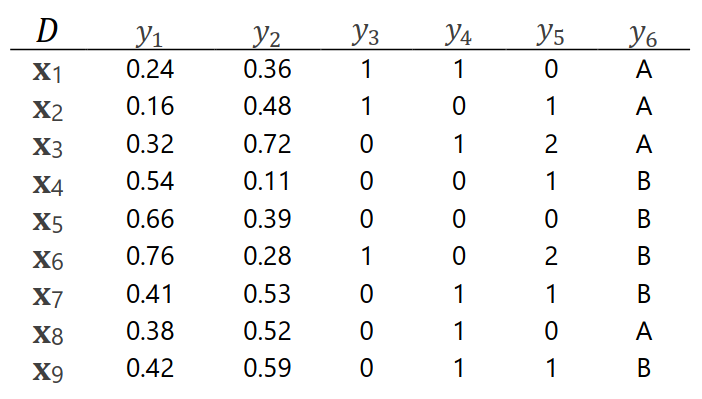
\includegraphics[width=9cm]{./assets/dataset_d.png}
  \label{fig:PartI-dataset-d}
\end{figure}

\begin{enumerate}[leftmargin=\labelsep]
  \item \textbf{Consider $x_1$ - $x_7$ to be training observations, $x_8$ - $x_9$ to be testing observations, $y_1$ - $y_5$ to be input
          variables and $y_6$ to be the target variable.\\
          \textit{Hint}: you can use \texttt{scipy.stats.multivariate\_normal} for multivariate distribution calculus}
        \begin{enumerate}
          \item \textbf{Learn a Bayesian classifier assuming: i) $\{y_1, y_2\}$, $\{y_3, y_4\}$ and $\{y_5\}$ sets of independent
                  variables (e.g., $y_1 \ind y_3$ yet $y_1 \not\!\ind y_2$), and ii) $y_1 \times y_2 \in \mathbb{R}^{2}$ is normally distributed. Show all
                  parameters (distributions and priors for subsequent testing).}

                \vskip 0.3cm
                As stated by the question prompt, variable sets \(\left\{y_1, y_2\right\}\), \(\left\{y_3, y_4\right\}\) and \(\left\{y_5\right\}\) are independent.
                Since we have seven training observations, we will use those to train a Bayesian classifier.

                We will refer to the outcome, which can be A or B, as class, or simply as c.

                To estimate $P(\text{class} | y_1, y_2, y_3, y_4, y_5)$, we can use Bayes' theorem:

                \begin{equation}\label{ex1-bayes1}
                  P(\text{class}| y_1, y_2, y_3, y_4, y_5) = \frac{P(y_1, y_2, y_3, y_4, y_5 | \text{class}) \times P(\text{class})}{P(y_1, y_2, y_3, y_4, y_5)}
                \end{equation}

                Since we know $\left\{y_1, y_2\right\}$, $\left\{y_3, y_4\right\}$ and $\left\{y_5\right\}$ are independent,
                we can rewrite $P(y_1, y_2, y_3, y_4, y_5)$ as $P(y_1, y_2) \cdot P(y_3, y_4) \cdot P(y_5)$.
                Rewriting \eqref{ex1-bayes1} with this, results in:

                \begin{equation}\label{ex1-bayes2}
                  P(\text{class}| y_1, y_2, y_3, y_4, y_5) = \frac{P(y_1, y_2 | \text{class}) P(y_3, y_4 | \text{class}) P(y_5 | \text{class}) \times P(\text{class})}{P(y_1, y_2)P(y_3, y_4)P(y_5)}
                \end{equation}

                Given a new observation $O$, we are able to classify it by calculating $P(\text{class}|O)$ for all classes and selecting the class with the
                highest probability as our prediction.

                \begin{equation}\label{ex1-map}
                  \begin{aligned}
                    \hat{z} & = \underset{c \in \{A, B\}}{\text{arg max}} \medspace \left\{P(\text{c} | O)\right\}                                                                               \\
                            & = \underset{c \in \{A, B\}}{\text{arg max}} \medspace \left\{\frac{P(y_1, y_2 | c) P(y_3, y_4 | c) P(y_5 | c) \times P(c)}{P(y_1, y_2) P(y_3, y_4) P(y_5)}\right\} \\
                            & = \underset{c \in \{A, B\}}{\text{arg max}} \medspace \left\{P(y_1, y_2 | c) P(y_3, y_4 | c) P(y_5 | c) \times P(c)\right\}
                            & \parbox{15em}{(we can remove parameters that do not depend on $c$)}
                  \end{aligned}
                \end{equation}

                We can now begin to compute these parameters.

                \textbf{Note:} Even though $P(y_1, y_2)$, $P(y_3, y_4)$ and $P(y_5)$ are not necessary
                to apply the model, we will still calculate them for the sake of showing
                all parameters.

                Calculating $P(\text{A})$, $P(\text{B})$ and all parameters involving $y_1$ through
                $y_5$ is straightforward, since they can be infered from the table.

                We have 3 observations of A and 4 observations of B, out of a total of 7 training observations.
                Therefore,

                \[
                  \begin{array}{cc}
                    P(\text{A}) = \frac{3}{7} &
                    P(\text{B}) = \frac{4}{7}
                  \end{array}
                \]

                In a similiar manner we can obtain the probabilities for $y_5$,

                \[
                  \begin{array}{ccc}
                    P(y_5 = 0) = \frac{2}{7} &
                    P(y_5 = 1) = \frac{3}{7} &
                    P(y_5 = 2) = \frac{2}{7}
                  \end{array}
                \]

                Now for the conditional probabilities of $y_5$,

                \[
                  \begin{array}{ccc}
                    P(y_5 = 0 \ | \text{A}) = \frac{1}{3}, &
                    P(y_5 = 1 \ | \text{A}) = \frac{1}{3}, &
                    P(y_5 = 2 \ | \text{A}) = \frac{1}{3}    \\[\medskipamount]
                    P(y_5 = 0 \ | \text{B}) = \frac{1}{4}, &
                    P(y_5 = 1 \ | \text{B}) = \frac{2}{4}, &
                    P(y_5 = 2 \ | \text{B}) = \frac{1}{4}
                  \end{array}
                \]

                For the four possible combinations of $y_3$ and $y_4$ we can follow
                the same logic as above,

                \[
                  \begin{array}{cc}
                    P(y_3 = 0, \ y_4 = 0) = \frac{2}{7}, &
                    P(y_3 = 0, \ y_4 = 1) = \frac{2}{7}    \\[\medskipamount]
                    P(y_3 = 1, \ y_4 = 0) = \frac{2}{7}, &
                    P(y_3 = 1, \ y_4 = 1) = \frac{1}{7}
                  \end{array}
                \]

                Finally, considering each class and the four possible combinations
                of $y_3$ and $y_4$, we can use the table to calculate the following:

                \[
                  \begin{array}{cc}
                    P(y_3 = 0, \ y_4 = 0 \ | \text{A}) = \frac{0}{3}, &
                    P(y_3 = 0, \ y_4 = 1 \ | \text{A}) = \frac{1}{3}    \\[\medskipamount]
                    P(y_3 = 1, \ y_4 = 0 \ | \text{A}) = \frac{1}{3}, &
                    P(y_3 = 1, \ y_4 = 1 \ | \text{A}) = \frac{1}{3}
                  \end{array}
                \]

                \[
                  \begin{array}{cc}
                    P(y_3 = 0, \ y_4 = 0 \ | \text{B}) = \frac{2}{4}, &
                    P(y_3 = 0, \ y_4 = 1 \ | \text{B}) = \frac{1}{4}    \\[\medskipamount]
                    P(y_3 = 1, \ y_4 = 0 \ | \text{B}) = \frac{1}{4}, &
                    P(y_3 = 1, \ y_4 = 1 \ | \text{B}) = \frac{0}{4}
                  \end{array}
                \]

                Calculating now the parameters related to the variable set $\left\{y_1, y_2\right\}$. We know that $(y_1, y_2)$ follows a Multivariate Gaussian Distribution.
                Therefore,

                \begin{equation}\label{ex1-normal}
                  P\left((y_1, y_2) | \boldsymbol{\mu}, \Sigma\right)
                  = \mathcal{N}\left((y_1, y_2) | \boldsymbol{\mu}, \Sigma\right)
                \end{equation}

                We can use the observations we have to approximate a value for the
                2-dimensional mean vector ($\boldsymbol{\mu}$) and the covariance matrix ($\Sigma$).

                $$
                  \begin{aligned}
                    \boldsymbol{\mu} = \frac{1}{7} \sum^{7}_{i=1} \begin{bmatrix}y_{1,i} \\y_{2,i} \\\end{bmatrix} & =
                    \frac{1}{7}
                    \left(\begin{bmatrix}0.24 \\0.36 \\\end{bmatrix} +
                    \begin{bmatrix}0.16 \\0.48 \\\end{bmatrix} +
                    \begin{bmatrix}0.32 \\0.72 \\\end{bmatrix} +
                    \begin{bmatrix}0.54 \\0.11 \\\end{bmatrix} +
                    \begin{bmatrix}0.66 \\0.39 \\\end{bmatrix} +
                    \begin{bmatrix}0.76 \\0.28 \\\end{bmatrix} +
                    \begin{bmatrix}0.41 \\0.53 \\\end{bmatrix}\right)                                                                                               \\
                                                                                                                   & = \begin{bmatrix}0.4414 \\0.41 \\\end{bmatrix}
                  \end{aligned}
                $$
                $$
                  \begin{aligned}
                    \Sigma_{00} & = \frac{1}{N-1} \sum^{N}_{i=1} (y_{1,i} - \mu_{1})^2 = \frac{1}{7-1} \left[(0.24-0.4414)^2 + \dots + (0.41-0.4414)^2\right] \approx 0.0491 \\
                    \Sigma_{11} & = \frac{1}{N-1} \sum^{N}_{i=1} (y_{2,i} - \mu_{2})^2 = \frac{1}{7-1} \left[(0.36-0.41)^2 + \dots + (0.53-0.41)^2\right] \approx 0.0375     \\
                    \Sigma_{01} & = \Sigma_{10} = \frac{1}{N-1} \sum^{N}_{i=1} (y_{1,i} - \mu_{1})(y_{2,i} - \mu_{2})                                                        \\
                                & = \frac{1}{7-1} \left[(0.24-0.4414)(0.36-0.41) + \dots + (0.41-0.4414)(0.53-0.41)\right]                                                   \\
                                & \approx -0.0211
                  \end{aligned}
                $$
                $$
                  \begin{aligned}
                    \Sigma & = \begin{bmatrix}\Sigma_{00} & \Sigma_{10}\\ \Sigma_{01} & \Sigma_{11}\end{bmatrix} = \begin{bmatrix}0.0491 & -0.0211 \\-0.0211 & 0.0375 \\\end{bmatrix}
                  \end{aligned}
                $$

                Therefore, $P(y_1, y_2) \sim \mathcal{N}\left((y_1, y_2) | \boldsymbol{\mu} = \begin{bmatrix}0.4414 \\0.41 \\\end{bmatrix},
                  \Sigma = \begin{bmatrix}0.0491 & -0.0211 \\-0.0211 & 0.0375 \\\end{bmatrix}\right)$.

                We can repeat the process for both classes (A and B).\\
                Starting with A:

                $$
                  \begin{aligned}
                    \boldsymbol{\mu} = \frac{1}{3} \sum^{3}_{i=1} \begin{bmatrix}y_{1,i} | \text{A} \\y_{2,i} | \text{A} \\\end{bmatrix} & =
                    \frac{1}{3}
                    \left(\begin{bmatrix}0.24 \\0.36 \\\end{bmatrix} +
                    \begin{bmatrix}0.16 \\0.48 \\\end{bmatrix} +
                    \begin{bmatrix}0.32 \\0.72 \\\end{bmatrix}\right)
                    = \begin{bmatrix}0.24 \\0.52 \\\end{bmatrix}
                  \end{aligned}
                $$
                $$
                  \begin{aligned}
                    \Sigma_{00} & = \frac{1}{N-1} \sum^{N}_{i=1} (y_{1,i} | \text{A} - \mu_{1})^2 = \frac{1}{3-1} \left[(0.24-0.24)^2 + \dots + (0.32-0.24)^2\right] \approx 0.0064 \\
                    \Sigma_{11} & = \frac{1}{N-1} \sum^{N}_{i=1} (y_{2,i} | \text{A} - \mu_{2})^2 = \frac{1}{3-1} \left[(0.36-0.52)^2 + \dots + (0.72-0.52)^2\right] \approx 0.0336 \\
                    \Sigma_{01} & = \Sigma_{10} = \frac{1}{N-1} \sum^{N}_{i=1} (y_{1,i} | \text{A} - \mu_{1})(y_{2,i} | \text{A} - \mu_{2})                                         \\
                                & = \frac{1}{3-1} \left[(0.24-0.24)(0.36-0.52) + \dots + (0.32-0.24)(0.72-0.52)\right] \approx 0.0096
                  \end{aligned}
                $$
                $$
                  \begin{aligned}
                    \Sigma & = \begin{bmatrix}\Sigma_{00} & \Sigma_{10}\\ \Sigma_{01} & \Sigma_{11}\end{bmatrix} = \begin{bmatrix}0.0064 & 0.0096 \\0.0096 & 0.0336 \\\end{bmatrix}
                  \end{aligned}
                $$

                Therefore, $P(y_1, y_2|\text{A}) \sim \mathcal{N}\left((y_1, y_2) | \boldsymbol{\mu} = \begin{bmatrix}0.24 \\0.52 \\\end{bmatrix},
                  \Sigma = \begin{bmatrix}0.0064 & 0.0096 \\0.0096 & 0.0336 \\\end{bmatrix}\right)$.

                And now the B:

                $$
                  \begin{aligned}
                    \boldsymbol{\mu} = \frac{1}{4} \sum^{4}_{i=1} \begin{bmatrix}y_{1,i} | \text{B} \\y_{2,i} | \text{B} \\\end{bmatrix} & =
                    \frac{1}{4}
                    \left(\begin{bmatrix}0.54 \\0.11 \\\end{bmatrix} +
                    \begin{bmatrix}0.66 \\0.39 \\\end{bmatrix} +
                    \begin{bmatrix}0.76 \\0.28 \\\end{bmatrix} +
                    \begin{bmatrix}0.41 \\0.53 \\\end{bmatrix}\right)
                    = \begin{bmatrix}0.5925 \\0.3275 \\\end{bmatrix}
                  \end{aligned}
                $$
                $$
                  \begin{aligned}
                    \Sigma_{00} & = \frac{1}{N-1} \sum^{N}_{i=1} (y_{1,i} | \text{B} - \mu_{1})^2 = \frac{1}{4-1} \left[(0.54-0.5925)^2 + \dots + (0.41-0.5925)^2\right] \approx 0.0229 \\
                    \Sigma_{11} & = \frac{1}{N-1} \sum^{N}_{i=1} (y_{2,i} | \text{B} - \mu_{2})^2 = \frac{1}{4-1} \left[(0.11-0.3275)^2 + \dots + (0.53-0.3275)^2\right] \approx 0.0315 \\
                    \Sigma_{01} & = \Sigma_{10} = \frac{1}{N-1} \sum^{N}_{i=1} (y_{1,i} | \text{B} - \mu_{1})(y_{2,i} | \text{B} - \mu_{2})                                             \\
                                & = \frac{1}{4-1} \left[(0.54-0.5925)(0.11-0.3275) + \dots + (0.41-0.5925)(0.53-0.3275)\right] \approx -0.0098
                  \end{aligned}
                $$
                $$
                  \begin{aligned}
                    \Sigma & = \begin{bmatrix}\Sigma_{00} & \Sigma_{10}\\ \Sigma_{01} & \Sigma_{11}\end{bmatrix} = \begin{bmatrix}0.0229 & -0.0098 \\-0.0098 & 0.0315 \\\end{bmatrix}
                  \end{aligned}
                $$

                Therefore, $P(y_1, y_2|\text{B}) \sim \mathcal{N}\left((y_1, y_2) | \boldsymbol{\mu} = \begin{bmatrix}0.5925 \\0.3275 \\\end{bmatrix},
                  \Sigma = \begin{bmatrix}0.0229 & -0.0098 \\-0.0098 & 0.0315 \\\end{bmatrix}\right)$.

                We now have all the parameters necessary to apply the Bayesian classifier to new observations.

          \item \textbf{Under a MAP assumption, classify each testing observation showing all of your calculus.} \label{ex:1b}

                \vskip 0.3cm
                Since we will need the ($y_1$, $y_2$) pdf values for the following exercises, let's calculate them using \texttt{scipy.multivariate\_normal}, just like it was suggested in the hint:

                \lstinputlisting[language=Python]{./assets/code_multivariate_normal.py}

                From the code above we get the following:
                \[
                  \begin{array}{cc}
                    P(y_1 = 0.38, y_2 = 0.52) \approx 3.6225, &
                    P(y_1 = 0.42, y_2 = 0.59) \approx 2.5387
                  \end{array}
                \]
                \[
                  \begin{array}{cc}
                    P(y_1 = 0.38, y_2 = 0.52 | A) \approx 0.9847, &
                    P(y_1 = 0.38, y_2 = 0.52 | B) \approx 1.9623    \\[\medskipamount]
                    P(y_1 = 0.42, y_2 = 0.59 | A) \approx 0.4031, &
                    P(y_1 = 0.42, y_2 = 0.59 | B) \approx 1.7285
                  \end{array}
                \]

                Since we are under a Maximum a Posteriori assumption, we can just use the expression at \eqref{ex1-map}
                and replace the values for each of the testing observations ($x_8$ and $x_9$).\\
                \textbf{Starting} with $x_8$:
                $$
                  \begin{aligned}
                    P(y_1 = 0.38, y_2 = 0.52 | A) P(y_3 = 0, y_4 = 1 | A) P(y_5 = 0 | A) \times P(A) & = 0.9847 \times \frac{1}{3} \times \frac{1}{3} \times \frac{3}{7} \approx 0.04689 \\
                    P(y_1 = 0.38, y_2 = 0.52 | B) P(y_3 = 0, y_4 = 1 | B) P(y_5 = 0 | B) \times P(B) & = 1.9623 \times \frac{1}{4} \times \frac{1}{4} \times \frac{4}{7} \approx 0.07008
                  \end{aligned}
                $$
                $$
                  \begin{aligned}
                    \hat{z}_{x_8} & = \underset{c \in \{A, B\}}{\text{arg max}} \medspace \left\{P(y_1 = 0.38, y_2 = 0.52 | c) P(y_3 = 0, y_4 = 1 | c) P(y_5 = 0 | c) \times P(c)\right\}    \\
                                  & = \text{arg max} \medspace \left\{P(y_1, y_2 | A) P(y_3, y_4 | A) P(y_5 | A) \times P(A); P(y_1, y_2 | B) P(y_3, y_4 | B) P(y_5 | B) \times P(B)\right\} \\
                                  & = B
                  \end{aligned}
                $$

                And \textbf{now} with $x_9$:
                $$
                  \begin{aligned}
                    P(y_1 = 0.42, y_2 = 0.59 | A) P(y_3 = 0, y_4 = 1 | A) P(y_5 = 1 | A) \times P(A) & = 0.4031 \times \frac{1}{3} \times \frac{1}{3} \times \frac{3}{7} \approx 0.0192 \\
                    P(y_1 = 0.42, y_2 = 0.59 | B) P(y_3 = 0, y_4 = 1 | B) P(y_5 = 1 | B) \times P(B) & = 1.7285 \times \frac{1}{4} \times \frac{2}{4} \times \frac{4}{7} \approx 0.1235
                  \end{aligned}
                $$
                $$
                  \begin{aligned}
                    \hat{z}_{x_9} & = \underset{c \in \{A, B\}}{\text{arg max}} \medspace \left\{P(y_1 = 0.42, y_2 = 0.59 | c) P(y_3 = 0, y_4 = 1 | c) P(y_5 = 1 | c) \times P(c)\right\}    \\
                                  & = \text{arg max} \medspace \left\{P(y_1, y_2 | A) P(y_3, y_4 | A) P(y_5 | A) \times P(A); P(y_1, y_2 | B) P(y_3, y_4 | B) P(y_5 | B) \times P(B)\right\} \\
                                  & = B
                  \end{aligned}
                $$

                \textbf{Therefore}, we conclude that under a MAP assumption, observations $x_8$ and $x_9$ will be classified with B and B, respectively.

          \item \textbf{Consider that the default decision threshold of $\theta = 0.5$ can be adjusted according to}

                \[
                  f(\textbf{x}|\theta)=
                  \begin{cases}
                    A, & P(A|\textbf{x}) > \theta \\
                    B, & \text{otherwise}
                  \end{cases}
                \]

                \textbf{Under a maximum likelihood assumption, what thresholds optimize testing accuracy?}

                \vskip 0.3cm
                Since we know that $P(A|y_1, y_2, y_3, y_4, y_5) + P(B|y_1, y_2, y_3, y_4, y_5)$ must be equal to 1, we need to normalize the values.
                Therefore, we get these new updated values for the posteriors:

                \begin{equation}\label{exI1-c-N}
                  \begin{aligned}
                    P(A|y_1, y_2, y_3, y_4, y_5) & = \frac{P(A|y_1, y_2, y_3, y_4, y_5)}{P(A|y_1, y_2, y_3, y_4, y_5) \ + \ P(B|y_1, y_2, y_3, y_4, y_5)} \\
                    P(B|y_1, y_2, y_3, y_4, y_5) & = \frac{P(B|y_1, y_2, y_3, y_4, y_5)}{P(B|y_1, y_2, y_3, y_4, y_5) \ + \ P(A|y_1, y_2, y_3, y_4, y_5)}
                  \end{aligned}
                \end{equation}

                \textbf{Note:} To make the equations easier to read, we simplified "$y_1 = 0.38, \ y_2 = 0.52, \ y_3 = 0, \ y_4 = 1, \ y_5 = 0$" by only writing "$x_8$"
                and "$y_1 = 0.42, \ y_2 = 0.59, \ y_3 = 0, \ y_4 = 1, \ y_5 = 1$" by only writing "$x_9$", given that those variable values characterize each observation.

                \text{On question \hyperref[ex:1b]{1.b)} we calculated the following values:}
                \[
                  \begin{array}{cc}
                    P(A) = \frac{3}{7}, &
                    P(B) = \frac{4}{7}
                  \end{array}
                \]
                \[
                  \begin{array}{cc}
                    P(x_8 | A) \times P(A) \approx 0.04689, &
                    P(x_8 | B) \times P(B) \approx 0.07008    \\[\medskipamount]
                    P(x_9 | A) \times P(A) \approx 0.0192,  &
                    P(x_9 | B) \times P(B) \approx 0.1235
                  \end{array}
                \]

                \textbf{Note:} According to the \textit{FAQ}, we can use the \textbf{likelihood} as a \textbf{rough proxy for posteriors}.
                Therefore, we will proceed with the assumption that $P(x | A)$ roughly estimates $P(A | x)$, implying that the likelihood
                will serve as an approximation for the posteriors used to calibrate the threshold.

                Hence why, we need to calculate the likelihoods:
                $$
                  \begin{array}{cc}
                    P(x_8 | A) = 0.10941, &
                    P(x_8 | B) = 0.12264    \\[\medskipamount]
                    P(x_9 | A) = 0.0448,  &
                    P(x_9 | B) = 0.216125
                  \end{array}
                $$

                To obtain the posterior values, we simply substitute the previously calculated values into the formula at equation \eqref{exI1-c-N} to normalize them.
                As stated before, we are assuming $P(A | x) \approx P(x | A)$ and $P(B | x) \approx P(x | B)$:
                $$
                  \begin{array}{cc}
                    P(A | x_8) = \frac{0.10941}{0.10941 + 0.12264} \approx 0.4715 &
                    P(B | x_8) = \frac{0.12264}{0.12264 + 0.10941} \approx 0.5285   \\[\medskipamount]
                    P(A | x_9) = \frac{0.0448}{0.0448 + 0.216125} \approx 0.1717  &
                    P(B | x_9) = \frac{0.216125}{0.216125 + 0.0448} \approx 0.8283
                  \end{array}
                $$

                As observed, we now have $P(A | x_8) + P(B | x_8) = 1$ and $P(A | x_9) + P(B | x_9) = 1$, indicating that we have obtained normalized probabilities.

                Our goal is to get optimal testing accuracy of 100\%. To accomplish this, we have to look into the accuracy formula, given by:
                $$
                  \text{accuracy} = \frac{\text{TP} + \text{TN}}{\text{TP} + \text{FP} + \text{TN} + \text{FN}}
                $$

                For the fraction to be of value 1, our observations need to be only true positives and true negatives. Therefore, we need observations $x_8$ and $x_9$ to be classified as A and B, respectively.
                This leads to the conclusion that the following inequalities, when solved will yield us the interval of values that the threshold ($\theta$) can take so that the accuracy is 100\%.
                \[
                  \begin{aligned}
                    P(A | x_8) & > \theta \Rightarrow x_8 \ \text{gets classified as A}    \\
                    P(A | x_9) & \leq \theta \Rightarrow x_9 \ \text{gets classified as B}
                  \end{aligned}
                \]
                \begin{equation}
                  P(A | x_9) \leq \theta < P(A | x_8) \Rightarrow 0.1717 \leq \theta < 0.4715 \Rightarrow \theta \in [0.1717, 0.4715[
                \end{equation}

        \end{enumerate}

  \item \textbf{Let $y_1$ be the target numeric variable, $y_2$ - $y_6$ be the input variables where $y_2$ is binarized under an
          equal-width (equal-range) discretization. For the evaluation of regressors, consider a 3-fold
          cross-validation over the full dataset ($x_1$ - $x_9$) without shuffling the observations.}
        \begin{enumerate}
          \item \textbf{Identify the observations and features per data fold after the binarization procedure.}

                \vskip 0.3cm
                To do the \textbf{binarization procedure} with an \textbf{equal-width discretization}, we need to divide $y_2$ into two intervals. Which are:

                \[
                  \begin{array}{cc}
                    \text{interval}_1 = [0, 0.5] & \quad
                    \text{interval}_2 = [0.5, 1]
                  \end{array}
                \]

                \textbf{Here is the binarization of $y_2$} based on those intervals:
                \begin{center}
                  \begin{tabular}{c|cccccc}
                    \(D\)   & \(y_1\) & \(y_2\) & \(y_3\) & \(y_4\) & \(y_5\) & \(y_6\) \\
                    \hline
                    \(x_1\) & 0.24    & 0       & 1       & 1       & 0       & A       \\
                    \(x_2\) & 0.16    & 0       & 1       & 0       & 1       & A       \\
                    \(x_3\) & 0.32    & 1       & 0       & 1       & 2       & A       \\
                    \(x_4\) & 0.54    & 0       & 0       & 0       & 1       & B       \\
                    \(x_5\) & 0.66    & 0       & 0       & 0       & 0       & B       \\
                    \(x_6\) & 0.76    & 0       & 1       & 0       & 2       & B       \\
                    \(x_7\) & 0.41    & 1       & 0       & 1       & 1       & B       \\
                    \(x_8\) & 0.38    & 1       & 0       & 1       & 0       & A       \\
                    \(x_9\) & 0.42    & 1       & 0       & 1       & 1       & B       \\
                  \end{tabular}
                \end{center}

                \textbf{Subsequently}, we proceed to determine our folds. In this case, we will have three folds, each containing three observations.
                This choice aligns with the prompt instructions of using a 3-fold cross-validation approach.
                \[
                  \begin{array}{ccc}
                    \text{Fold}_1 = x_1 \medspace x_2 \medspace x_3 & \quad
                    \text{Fold}_2 = x_4 \medspace x_5 \medspace x_6 & \quad
                    \text{Fold}_3 = x_7 \medspace x_8 \medspace x_9
                  \end{array}
                \]

                \textbf{So} our datasets will be:

                \begin{table}[H]
                  \centering

                  \begin{minipage}{.4\linewidth}
                    \centering
                    {\bfseries\strut Fold 1}
                    \begin{tabular}{c|cccccc}
                      \(D\)   & \(y_1\) & \(y_2\) & \(y_3\) & \(y_4\) & \(y_5\) & \(y_6\) \\
                      \hline
                      \(x_1\) & 0.24    & 0       & 1       & 1       & 0       & A       \\
                      \(x_2\) & 0.16    & 0       & 1       & 0       & 1       & A       \\
                      \(x_3\) & 0.32    & 1       & 0       & 1       & 2       & A       \\
                    \end{tabular}
                  \end{minipage}
                  \quad
                  \begin{minipage}{.4\linewidth}
                    \centering
                    {\bfseries\strut Fold 2}
                    \begin{tabular}{c|cccccc}
                      \(D\)   & \(y_1\) & \(y_2\) & \(y_3\) & \(y_4\) & \(y_5\) & \(y_6\) \\
                      \hline
                      \(x_4\) & 0.54    & 0       & 0       & 0       & 1       & B       \\
                      \(x_5\) & 0.66    & 0       & 0       & 0       & 0       & B       \\
                      \(x_6\) & 0.76    & 0       & 1       & 0       & 2       & B       \\
                    \end{tabular}
                  \end{minipage}

                  \vskip 0.3cm
                  \begin{minipage}{.4\linewidth}
                    \centering
                    {\bfseries\strut Fold 3}
                    \begin{tabular}{c|cccccc}
                      \(D\)   & \(y_1\) & \(y_2\) & \(y_3\) & \(y_4\) & \(y_5\) & \(y_6\) \\
                      \hline
                      \(x_7\) & 0.41    & 1       & 0       & 1       & 1       & B       \\
                      \(x_8\) & 0.38    & 1       & 0       & 1       & 0       & A       \\
                      \(x_9\) & 0.42    & 1       & 0       & 1       & 1       & B       \\
                    \end{tabular}
                  \end{minipage}
                \end{table}

          \item \textbf{Consider a distance-weighted \textit{k}NN with k = 3, Hamming distance (\textit{d}), and 1 / \textit{d} weighting.
                  Compute the MAE of this \textit{k}NN regressor for the $1^{st}$ iteration of the cross-validation (i.e. train
                  observations have the lower indices).}

                \vskip 0.3cm

                The formula for the \textbf{weight} ($w_i$) and the \textbf{weighted average} ($f$), considering that k=3, are the following:

                \begin{equation}\label{exI2-a-WA}
                  \begin{array}{c|c}
                    \centering
                    w_i(x_{new})=
                    \begin{cases}
                      \frac{1}{d(x_{new},\; x_i)}, & x_{new} \neq x_i \\
                      1,                           & \text{otherwise}
                    \end{cases}
                    \quad &
                    \quad
                    \hat{z}_{x_{new}} = f(x_{new}) = \frac{\sum_{i=1}^{n} w_i(x_{new}) f(x_i)}{\sum_{i=1}^{n} w_i(x_{new})}
                  \end{array}
                \end{equation}

                And the formula for the \textbf{mean absolute error} is given by:

                \begin{equation}\label{exI2-a-MAE}
                  MAE(\hat{z}, z) = \frac{1}{n} \sum_{i=1}^{n} \left| z_i - \hat{z}_i \right|
                \end{equation}

                As stated in the prompt, we will use Folds 1 and 2 for training, reserving Fold 3 for testing. Let's start by computing
                the \textbf{Hamming distances}, for $x_7$, $x_8$ and $x_9$:

                \begin{center}
                  \begin{tabular}{c|cccccc}
                                   & \(x_1\)                        & \(x_2\) & \(x_3\)                        & \(x_4\)                        & \(x_5\)                        & \(x_6\) \\
                    \hline
                    \(H(x_7,x_j)\) & 4                              & 4       & \textcolor{Maroon}{\textbf{2}} & \textcolor{Maroon}{\textbf{2}} & \textcolor{Maroon}{\textbf{3}} & 4       \\
                    \(H(x_8,x_j)\) & \textcolor{Maroon}{\textbf{2}} & 4       & \textcolor{Maroon}{\textbf{1}} & 4                              & \textcolor{Maroon}{\textbf{3}} & 5       \\
                    \(H(x_9,x_j)\) & 4                              & 4       & \textcolor{Maroon}{\textbf{2}} & \textcolor{Maroon}{\textbf{2}} & \textcolor{Maroon}{\textbf{3}} & 4       \\
                  \end{tabular}
                \end{center}

                Now let's determine the \textbf{three closest neighbors} (lowest Hamming distance values) for each test observation:

                \begin{itemize}
                  \item For $x_7$ it is $x_3$, $x_4$ and $x_5$
                  \item For $x_8$ it is $x_1$, $x_3$ and $x_5$
                  \item For $x_9$ it is $x_3$, $x_4$ and $x_5$
                \end{itemize}

                The next step is calculating their \textbf{weighted average}. By replacing the
                formula on \eqref{exI2-a-WA}, we get the following values:

                $$
                  \begin{aligned}
                    \hat{z}_{x_7} & = f(x_7) = \frac{\frac{1}{2} \cdot 0.32 + \frac{1}{2} \cdot 0.54 + \frac{1}{3} \cdot 0.66}{\frac{1}{2} + \frac{1}{2} + \frac{1}{3}} = 0.4875 \\
                    \hat{z}_{x_8} & = f(x_8) = \frac{\frac{1}{2} \cdot 0.24 + \frac{1}{1} \cdot 0.32 + \frac{1}{3} \cdot 0.66}{\frac{1}{2} + \frac{1}{1} + \frac{1}{3}} = 0.36   \\
                    \hat{z}_{x_9} & = f(x_9) = \frac{\frac{1}{2} \cdot 0.32 + \frac{1}{2} \cdot 0.54 + \frac{1}{3} \cdot 0.66}{\frac{1}{2} + \frac{1}{2} + \frac{1}{3}} = 0.4875
                  \end{aligned}
                $$

                Now we have the estimates for the testing observations along with their real values:

                $$
                  \begin{aligned}
                    \hat{z} & = \left(\hat{z}_{x_7}, \hat{z}_{x_8}, \hat{z}_{x_9}\right) = \left(0.4875, 0.36, 0.4875\right) \\
                    z       & = \left(0.41, 0.38, 0.42\right)
                  \end{aligned}
                $$

                \textbf{Finally,} let's compute the mean absolute error by using the formula on \eqref{exI2-a-MAE}:

                \begin{equation*}
                  MAE(\hat{z}, z) = \frac{1}{3} \left( \left|0.41 - 0.4875\right| + \left|0.38 - 0.36\right| + \left|0.42 - 0.4875\right| \right) = 0.055
                \end{equation*}

        \end{enumerate}
\end{enumerate}

\vskip 0.5cm

\begin{center}
  \large{\textbf{Part II}: Programming and critical analysis}\normalsize
\end{center}

\noindent Considering the \texttt{column\_diagnosis.arff} dataset available at the course webpage’s homework tab. Using \texttt{sklearn}, apply a 10-fold stratified
cross-validation with shuffling (\texttt{random\_state=0}) for the assessment of predictive models along this section.

\begin{enumerate}[leftmargin=\labelsep]
  \item \textbf{Compare the performance of \textit{k}NN with k = 5 and Naïve Bayes with Gaussian assumption
          (consider all remaining parameters for each classifier as \texttt{sklearn}'s default):}
        \begin{enumerate}
          \item \textbf{Plot two boxplots with the fold accuracies for each classifier.}

                \vskip 0.3cm
                \lstinputlisting[language=Python]{./assets/code_1a.py}

                \begin{figure}[H]
                  \centering
                  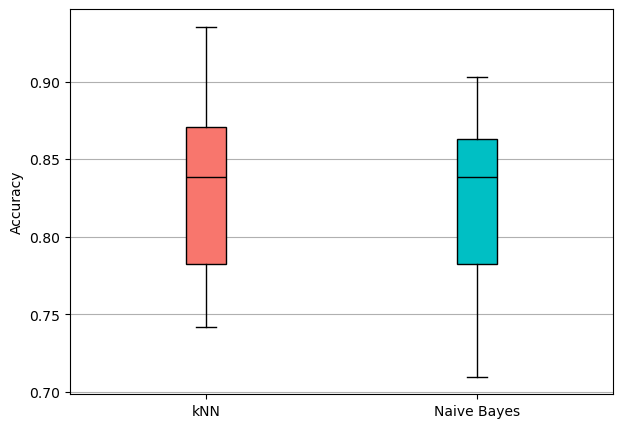
\includegraphics[width=13cm]{./assets/boxplot_ex1_PartII.png}
                  \caption{Boxplots with the fold accuracies of \textit{k}NN (k = 5) and Naïve Bayes}
                  \label{fig:PartII-ex1a}
                \end{figure}

          \item \textbf{Using \texttt{scipy}, test the hypothesis "\textit{k}NN is statistically superior to Naïve Bayes regarding
                  accuracy", asserting whether is true.}

                \vskip 0.3cm
                We will consider the null hypothesis and alternate hypothesis below and perform a right-tailed test using the accuracies
                obtained in the previous answer,

                $$
                  \begin{aligned}
                    H_0: & \;\; \text{accuracy}_{k\text{NN}} = \text{accuracy}_{\text{Naïve Bayes}} \\
                    H_1: & \;\; \text{accuracy}_{k\text{NN}} > \text{accuracy}_{\text{Naïve Bayes}}
                  \end{aligned}
                $$

                \lstinputlisting[language=Python]{./assets/code_1b.py}

                Using \texttt{scipy} we get a p-value of, approximately, 0.190428 = 19.0428 \%.

                This means we cannot reject the hypothesis $H_0$ at common significance levels (1\%, 5\% and 10\%).

                \textbf{Therefore,} we cannot assert that \textit{k}NN is statistically superior to Naïve Bayes. We also cannot
                state that the hypothesis on the statement is outright false without checking other statistical tests.
        \end{enumerate}

  \item \textbf{Consider two \textit{k}NN predictors with k = 1 and k = 5 (uniform weights, Euclidean distance,
          all remaining parameters as default). Plot the differences between the two cumulative confusion
          matrices of the predictors. Comment.}

        \vskip 0.3cm
        \lstinputlisting[language=Python]{./assets/code_2.py}

        \begin{figure}[H]
          \centering
          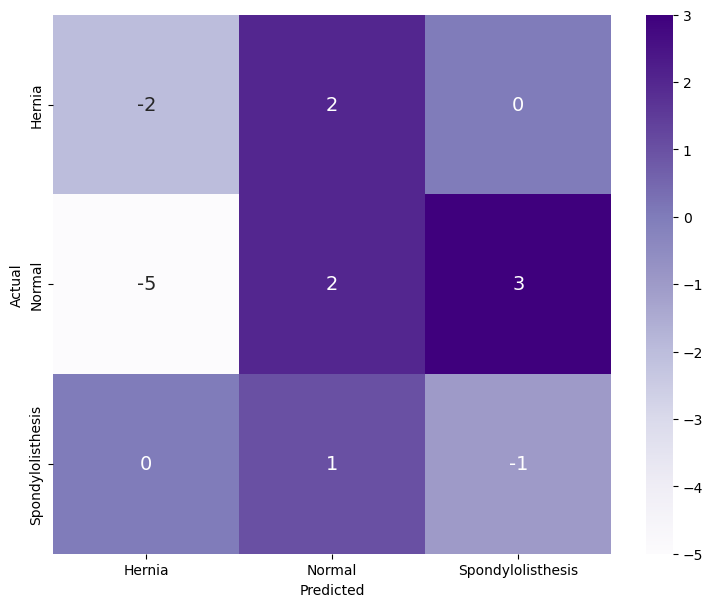
\includegraphics[width=13cm]{./assets/cumulative_heatmap_ex2_PartII.png}
          \caption{Confusion Matrix Differences Between k=1 and k=5 k-Nearest Neighbors (\textit{k}NN) Classifiers}
          \label{fig:PartII-ex2}
        \end{figure}

        Upon examination of the difference matrix derived from the cumulative confusion matrices, it is evident that the \textit{k}NN model
        with k=5 surpasses the performance of k=1.

        For each cell in this matrix, we can determine which model (k=1 or k=5) had the most observations by noting if
        the cell value is negative or positive. A positive value indicates that k=1 had the most observations, while
        a negative value indicates that k=5 was the one with more observations.

        This superiority of the k=5 model is shown by the negative sum of the main diagonal elements, signifying higher accuracy.
        Additionally, the fact that the sum of incorrect predictions (false positives and false negatives) is positive suggests that
        k=5 has fewer miss classifications.

        \textbf{Therefore}, utilizing k=5 appears to be the preferable choice over k=1 for this task.

  \item \textbf{Considering the unique properties of \texttt{column\_diagnosis}, identify three possible difficulties
          of Naïve Bayes when learning from the given dataset.}

        \vskip 0.3cm
        Here are three possible difficulties of Naïve Bayes when learning from the given dataset, in no particular order:

        \begin{itemize}
          \item To apply Naïve Bayes, we assume that all variables were independent of one another, which might not be case, thus explaining a
                potential problem that would hinder its accuracy. In medical datasets, like this one, it is common for attributes to have complex
                dependencies, which Naïve Bayes cannot account for.
          \item There may be an inadequacy of Gaussian assumption, because the data used (\texttt{column\_diagnosis.arff}) is not very big
                (around 300 observations, with only some being used for training), and so there might not be enough data for probability density
                function/probability mass function approximations.
          \item Probabilities are estimated based on the number of occurences on the given training data, and so there might be imbalanced
                number of occurences for some given class. This might affect the value of the prior, creating biases in a Maximum a Priori
                assumption.
        \end{itemize}
\end{enumerate}

\end{document}
